
%\begin{figure*}[!bt]
%	\begin{minipage}{4cm}
%		\centering
%		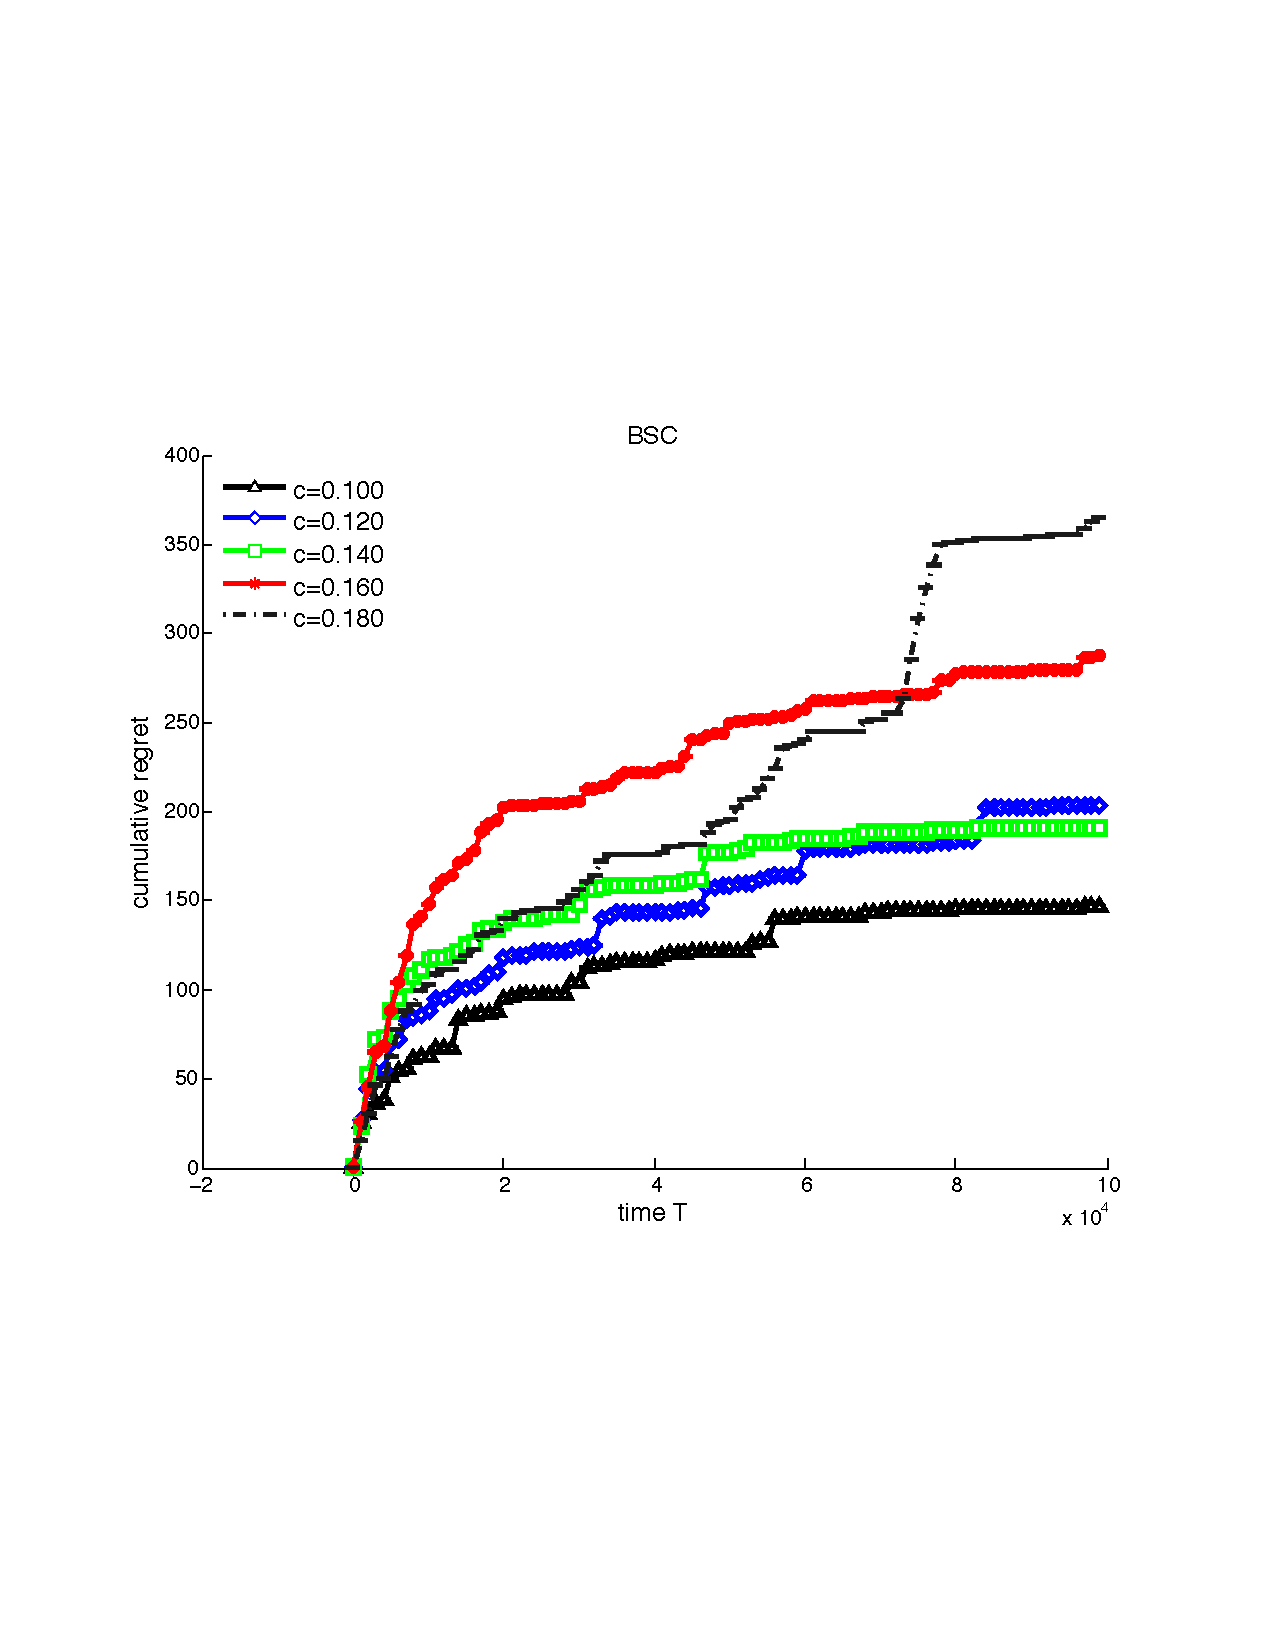
\includegraphics[scale=0.2]{../Simulations/Figures/BSC_SD}
%		\label{fig:BSC1}
%		\caption{BSC wtih SD}
%	\end{minipage}
%	\begin{minipage}{4cm}
%		\centering
%		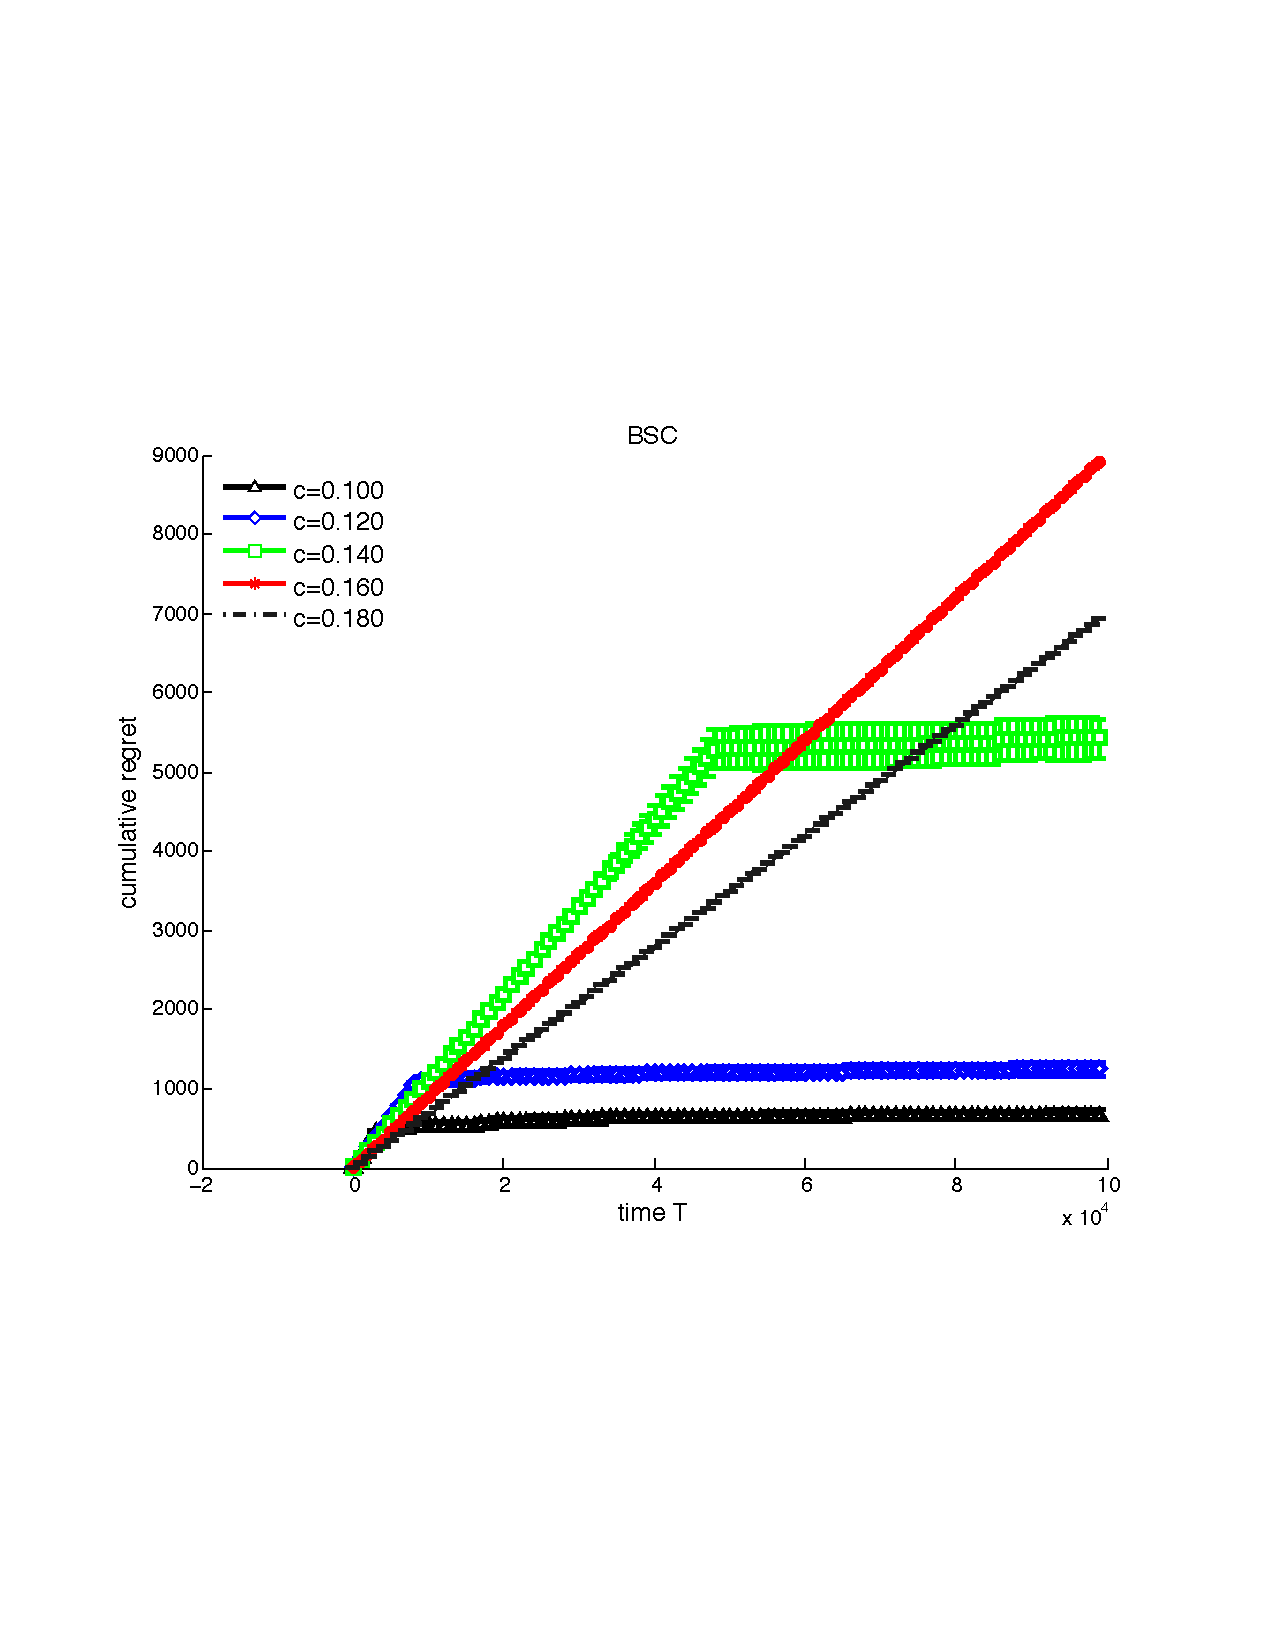
\includegraphics[scale=0.2]{../Simulations/Figures/BSC_WD}
%		\label{fig:BSC2}
%		\caption{BSC dataset}
%	\end{minipage}
%	\begin{minipage}{4cm}
%		\centering
%		\includegraphics[scale=0.2]{../Simulations/Figures/Heart}
%		\label{fig:Heart}
%		\caption{BSC dataset}
%	\end{minipage}
%	\begin{minipage}{4cm}
%		\centering
%		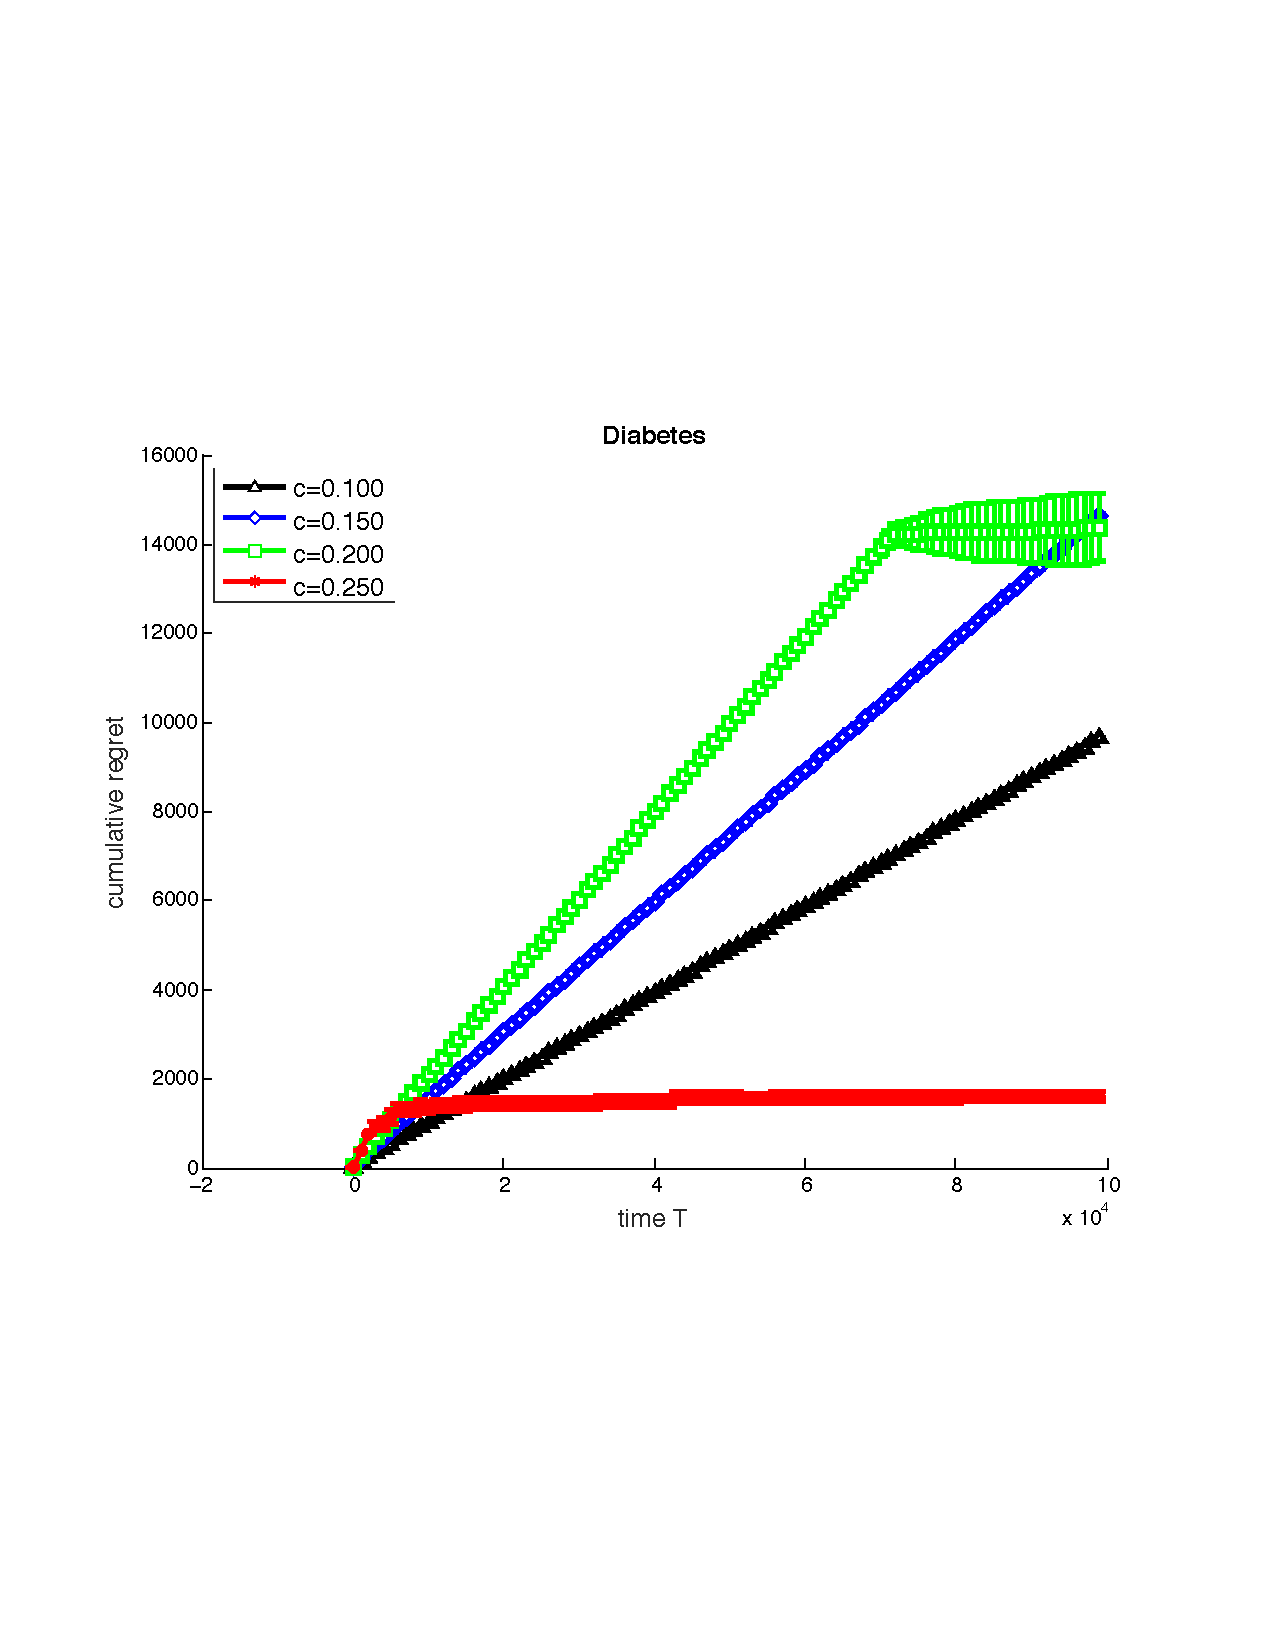
\includegraphics[scale=0.2]{../Simulations/Figures/Diabetes_WD}
%		\label{fig:Heart}
%		\caption{Heart dataset}
%	\end{minipage}
%	\vspace{.2cm}

%\noindent
%In Fig. \ref{fig:BSC1}, BSC data is generated that satisfies SD property and Algorithm \ref{alg:asym} is applied. In  Fig. \ref{fig:BSC2}, Algorithm \ref{alg:UCB} is applied on BSC data. In Fig. \ref{fig:BSC3}, true labels are used and standard UCB algorithm is applied on BSC dataset. In Fig. \ref{fig:Heart}, we applied Algorithm \ref{algo:UCB} on the heart dataset. 
%\end{figure*}

In this section we evaluate performance of \ref{alg:asym} and \ref{alg:UCB} on synthetic and real datasets (PIMA-Diabetes) and Heart Disease (Cleveland). Both of these datasets have accompanying costs for individual features.%. For synthetic example, we consider a binary symmetric channel, and for real world examples, we use diabetes (PIMA indiana) and heart disease (Clevland) from UCI dataset. In both datasets attributes/features are associated with costs, where features related to physical observations are cheap and that obtained from medical tests are costly. The experiments are setup as follows:

{\bf Synthetic:} we generate data as follows. The input, $Y_t$, is generated IID Ber($0.7$). Outputs for channels 1, 2, 3 have an overall error statistic, $\gamma_1 = 0.3,\,\gamma_2=0.3,\,\gamma=0.1$ respectively. To ensure SD we enforce Eq.~\ref{} during the generation process. To ensure WD we enforce Eq.~\ref{}.  %Channel $i=1,2,3$ flips input bit with probability $p_i$ where $p_1\geq p_2\geq p_3$. Transmission over channel $1$ is free and that over channel $2$ and $3$ costs price of $ c_2$ and $c_3\in (0,1] $ units per bit, respectively. Input bits are generated with probability $0.7$ and we set $p_1=.3, p_2=.1$ and $p_3=.05$.

{\bf Real Datatsets:} %we obtain a sensor acquisition setup from the datasets as follows: 
We split the features into three ``sensors'' based on their costs. For PIMA-Diabetes dataset (size = $768$) the first sensor is associated with patient history/profile with cost (\$ 6), the second sensor in addition utilizes a glucose-tolerance test (cost \$ 17) and the 2nd sensor input along with an insulin test (cost \$ 22). For the Heart dataset (size = $297$) we cluster patient profile and blood-pressure in to the first sensor (cost \$ 4 ), the second sensor in addition utilizes cholestrol readings, blood-sugar, and rest-ECG (Cost \$ 27) and the third sensor utilizes more extensive tests at a cost (\$ 500). 


We train three linear svm classifiers with slack cost with 5-fold cross-validation. The size of these datasets is relatively small and limits our ability to experiment. Therefore, after the classifiers are trained we re-sample data with replacement and generate a larger dataset of size $20000$. Note that Table~\ref{tab:ErrorTable1} shows that the resulting classifiers/tests on these datasets approximately satisfies SD condition and thus our setup should apply to these datasets. 
%
%
%The (linear, $C=.01$) are trained for each dataset, first one using only cheap features, second one  using cheap features plus few additional features and the third one using all features. These classifiers form sensors of a three stage SAP where classifier trained with cheap features is the first stage and that trained with all features forms the last stage. Cost of each stage is the sum of cost of features used to train that stage multiplied by a scaling factor $\lambda$ (trade-off parameter for accuracy and costs). Specific details for each dataset is given below.  
%
%{\bf PIMA indians diabetes} dataset consists of $768$ instances and has $8$ attributes. The labels identify if the instances are diabetic or not. $6$ of the attributes (age, sex, triceps, etc.) obtained from physical observations are cheap, and $2$ attributes (glucose and insulin) require expensive tests. First sensor of SAP is trained with $4$ cheap attributes and costs \$$4$. Second sensor is trained from $6$ attributes that cost \$$6$, and the last sesnor is trained with all $8$ attributes that cost \$$6$. We set $C_1= 4\lambda, C_2= 6\lambda$ and $C_3= 30\lambda$.
%
%{\bf Heart disease} dataset consists of $297$ instance (without missing values) and has $13$ attributes. $5$ class labels $(0,1,2,3,4)$ are mapped to binary values by taking value $0$ as `absence' of disease and values $(1,2,3,4)$ as `presence' of disease. First senor of SAP is trained with $4$ attributes which cost  \$$1$ each and second sensor is trained with $8$ attributes that cost \$$1$ each. Total cost of all attributes is \$$568$. We set $C_1= 7\lambda, C_2= 8\lambda$ and $C_3= 568\lambda$.
%
Various error probabilities for synthetic and datasets are listed in Table (\ref{tab:ErrorTable}).  
%The probabilities for the datasets are computed on $40 \%$ hold out data. 
	\begin{figure}[!h]
		\small
		\begin{tabular}[c]{c|c|c|c|c|c|c } 
			\label{tab:ErrorTable}
			%	\caption{cap:Error statistics}
			dataset & $\gamma_1$ & $\gamma_2$ & $\gamma_3$ &$\delta_{12}$ & $\delta_{13}$ & $\delta_{23}$ \\ \hline 
			BSC & .3 & .1 & .05 & .07 & .035 & .045\\  \hline
			diabetic & $0.345 $ & $ 0.324$ & 0.246 & $ 0.116 $ & 0.089 &0.058\\  \hline
			heart & $0.292$ & $0.27$ & 0.146 & $0.124$ & 0.067 & 0.079\\  \hline
		\end{tabular}
		\caption{Error statistics for real and synthetic datasets. $\delta_{ij}:=\P\{Y_j\neq Y \mid Y_i = Y\}$.}
\label{tab:error_stats}
	\end{figure}
To run the online algorithm, an instance is randomly selected from the dataset (with replacement) in each round and is input to the  algorithm. We repeat the experiments $20$ times (with different re-samplings of the datasets) to show variability of our experiments.

\noindent
{\bf Testing Learnability:}
We experiment with different USS algorithms on the synthetic dataset. Our purpose is twofold: (a) show the superior performance of reduction scheme (Alg~1) on SD and necessity of a more robust scheme to account for WD, (b) establish WD condition as the maximal learnable set.

\noindent
{\bf Unsupervised vs. Supervised Learning:}
The real datasets provide an opportunity to understand how different types of information can impact performance. We compare our USS algorithm (Alg.~\ref{alg:UCB}) against UCB bandit algorithms, where we obtain feedback of the reward (we consider both noisy and noiseless cases) for each action. Note that for USS we apply Alg.~2 because the real datasets does not satisfy SD condition. Our implementation for UCB algorithm is based on modification of Alg.~\ref{alg:UCB}) so that we keep track of actual pairwise error differences for each arm rather than pairwise-disagreements (Step 5 in Alg.~\ref{alg:UCB}). We benchmark the performance with respect to a budget constrained problem, where the objective is to pick a sensor that minimizes error with respect to a budget constraint. We consider both high and low available budget situations. For Heart and Diabetes datasets a low budget is about (\$ 10). We note from the error probabilities in Table~\ref{tab:error_stats} that the optimal sensor in such a situation is Sensor 1. On the other hand for a budget of about (\$ 50) the optimal sensor for Diabetes dataset is Sensor 3, while for the Heart dataset it is Sensor 2. To map this to our setting we consider an equivalent error-cost tradeoff objective ($\lambda$ Cost + Error) with an appropriate scaling parameter $\lambda$ so that it leads to the same sensor choice based on Eq.~\ref{eqn:interp_opt} as in the constrained one.


%This can also be seen from Eq.~\ref{}. Consequently, we choose an appropriate $\lambda$ that corresponds to the



%and the average is shown in figures (\ref{fig:BSC1}-\ref{fig:Heart}) with $95\%$ confidence bounds. The left Figure in\ref{fig: BSC1} we applied Algorithm \ref{alg:asym} on BSC data that satisfies SD property. As see, the algorithm learns the optimal arm. In Figure \ref{fig:BSC2} 
%we applied Algorithm \ref{alg:UCB} on BSC data where we fixed $c_1=0$ and $c_2+c_3=0.3$ while varying $c_2$ between $0.1$ $0.18$. For all the cost values, arm $2$ is optimal. When $c_2 \in \{0.1, 0.12,  0.14\}$ the weak dominance property is satisfied and the algorithm learns the optimal arm. For values $c_2 \in \{0.16, 0.18\}$ weak dominance property is violated we get linear regret as shown in the plots. In figure  \ref{fig:BSC3} we use the standard UCB algorithm that has access to the true labels and knows the if a sensor made error. As seen this setting learns much faster than than compared to unsupervised algorithm shown in figure \ref{fig:BSC1} and \ref{fig:BSC2}. In figure we apply Algorithm \ref{algo:UCB} on diabetes dataset varying the trade-off factor $\lambda$. In the regions where WD property holds, the algorithm identifies the optimal arm.